%!TEX root = ../main.tex
%%%%%%%%%%%%%%%%%%%%%%%%%%%%%%%%%%
% Links:
%
% Difficulty: Companies: 
%%%%%%%%%%%%%%%%%%%%%%%%%%%%%%%%%%


%\begin{figure} \centering
%   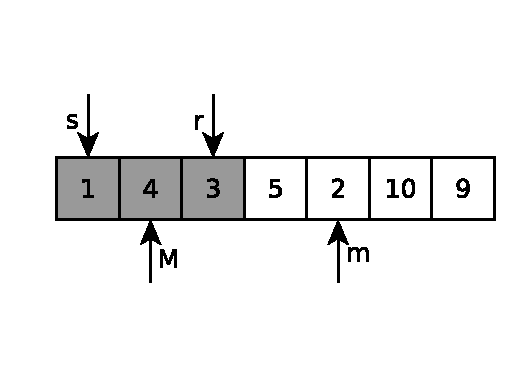
\includegraphics[width=\textwidth]{sources/max_num_chunks_sorted/images/example1}
%   \caption[Sample short cpation]{Sample Caption}. \label{fig:max_num_chunks_sorted:example1}
%   \end{figure}

\chapter{Sort the chunks, sort the array.}
\label{ch:max_num_chunks_sorted}
\section*{Introduction}

Sorting is a popular topic in computer science and in programming interviews. 
Its usefulness its beyond dispute and is it not surprising that there are literally
countless of research papers and algorithms on the topic. 

In this problem however we are not going to devise a novel sorting algorithm, instead 
will investigate how we can sort an entire array by sorting a number of its individual sub-arrays.
The idea is that we would like to know how we can split an array into pieces such that if each of the pieces is sorted 
individually then the final result would be equivalent to having sorted the entire array to begin with.

It is necessary to develop a key insight to solve this problem efficiently, 
and asking the right questions and looking at a number of good examples
is fundamental for doing so. In the next section we are going to explore how these insights 
can be gained and then turned into an efficient code. 

\section{Problem statement}
\begin{exercise}
\label{example:max_num_chunks_sorted:exercice1}
Write a function that given an array $I$ of integers returns the maximum number of sub-arrays (or chunks) of $I$ 
such that if each of the sub-array is sorted individually, then $I$ as a whole is sorted.

	%example1
	\begin{example}
		\label{example:max_num_chunks_sorted:example1}
		\hfill \\
		Given $I=\{45,88,1,9,90\}$ then the function return $1$.
		
	\end{example}

	%example2
	\begin{example}
		\label{example:max_num_chunks_sorted:example2}
		\hfill \\
		Given $I=\{4,3,2,1,5,9,10\}$ then the function return $4$. We can sort the following sub-arrays:
		\begin{itemize*}
			\item $[0,3]$
			\item $[4,4]$
			\item $[4,4]$
			\item $[4,4]$
		\end{itemize*}
	\end{example}
\end{exercise}

\section{Clarification Questions}

\begin{QandA}
	\item Can the chunks overlap? 
	\begin{answered}
		\textit{No. If you choose to sort two sub-arrays of $I$ $s_1=[p,q], p\leq q$ and $s_2=[x,y], x\leq y$ then either $x > q$ or $p>y$.}
	\end{answered}
	
\end{QandA}

\section{Discussion}
\label{max_num_chunks_sorted:sec:discussion}

\section{Brute-force}
\label{max_num_chunks_sorted:sec:bruteforce}


Let's start our discussion by thinking about a brute-force solution for this problem. 
One possible way of doing it would be to try to divide the array into $|I|$ parts, 
sort  them individually and then check if $I$ is sorted. 
If it is not we can try to divide $I$ into $|I|-1$ sub-arrays,
and check whether by sorting the resulting individual pieces $I$ turns to be sorted.
This line or reasoning can be generalized and a general brute-force approach
could work by progressively trying to split $I$ into less number of sub-arrays $k <|I|$.
For each of the possible  partitions of $I$ into $k$ subarrays, we can then check whether 
we can obtain a complete sorting of $I$ by only sorting the individual $k$ sub-arrays.
Eventually when $k=1$, $I$ would be sorted fully.

Clearly this algorithm is complete and correct
as all possible valid partitions of $I$ are checked. Its complexity is however exponential
in time as given a certain $k$ there are ${n \choose k} $ possible valid partition of $I$. 
Listing \ref{list:max_num_chunks_sorted:bruteforce} shows a C++ implementation of such idea. 


\begin{minipage}{\linewidth}
	\lstinputlisting[language=c++, caption={Bruteforce solution to the problem \textit{Sort the chunks, sort the array}.},label=list:max_num_chunks_sorted:bruteforce]{sources/max_num_chunks_sorted/max_num_chunks_sorted_solution1.cpp}
\end{minipage}


\section{Linear time}
\label{max_num_chunks_sorted:sec:lineartime}

\begin{minipage}{\linewidth}
	\lstinputlisting[language=c++, caption={Linear time solution to the problem \textit{Sort the chunks, sort the array}.},label=list:max_num_chunks_sorted]{sources/max_num_chunks_sorted/max_num_chunks_sorted_solution2.cpp}
\end{minipage}
